\documentclass{paper}
\usepackage{fullpage, amsmath, graphicx}

\title{\textbf{Regressions And Stuff}}

\author{}

\date{May 6, 2016}

\begin{document}
% \begin{titlepage}
% \centering
% Matei Zaharia\\
% TR 10\\
% May 6, 2016
% \end{titlepage}

\maketitle
\section{Introduction}

In this paper, we discuss various methods of calculating regression. First, we discuss the benfits of using Stochastic Gradient Descent versus Batch Gradient Descent. Next, we analyze the performance of these methods in performing a Least Squares Linear regression. Finally, we discuss blah blah

\section{Overview}


\section{Gradient Descent}

\emph{Gradient descent} is an iterative optimization algorithm; in other words, it calculates the parameters $\mathbf{x}$ that minimize a given objective function $f(\mathbf{x})$. The algorithm repeatedly translates an initial \emph{guess} $\mathbf{x}_0$ in a direction proportional to the negative \emph{gradient} $\nabla f(x)$.

In every step of the itreration, we update our guess as following:
\begin{align*}
\mathbf{x}_{n+1} = \mathbf{x} - \lambda \nabla f(\mathbf{x}_{n})
\end{align*}
where $\lambda$ is the \emph{step size} of the iteration. The algorithm terminates upon the following convergence condition: 
\begin{align*}
|f(\mathbf{x}_{n+1}) - f(\mathbf{x}_{n})| < \delta
\end{align*}
where $\delta$ is the convergence \emph{threshold}. Upon convergence, the algorithm returns a final guess of $\mathbf{x}_{\text{opt}} = \mathbf{x}_{n+1}$.

In this section, we compare two methods of gradient descent: \emph{batch gradient descent}, which computes a gradient over all samples for each iteration, and \emph{stochastic gradient descent}, which instead uses pointwise gradients.

To analyze the perforamnce of the different algorithms, we use the \emph{Gaussian function}:
\begin{align*}
f(x) = - \dfrac{1}{\sqrt{(2\pi)^n |\Sigma|}} \exp \left[-\dfrac{1}{2} (x - u)^T \Sigma^{-1} (x-u)\right]
\end{align*}
In addition, we use the \emph{quadratic bowl function}:
\begin{align*}
f(x) = \dfrac{1}{2} x^T A x - x^T b 
\end{align*}
Finally, we use the \emph{least squares error} function:
\begin{align*}
J(\theta) = |X\theta - y|^2
\end{align*}


\subsection{Batch Gradient Descent}

In batch gradient descent, for every iteration we calculate the gradient across the entire sample set. In this section, we analyze the affects of step size ($\lambda$), threshold ($\delta$), and initial guess $\mathbf{x}_{0}$ on the performance and accuracy of the gradient descent algorithm. 

First, we note that step size has a significant impact on the convergence rate of the algorithm. We run gradient descent on an arbitrary quadratic bowl function. As we increase the value of $\lambda$ from $0.0001$ to $0.001$, the magnitude of the gradient decreases more quickly, and the algorithm converges faster. Note that in this figure, all of the gradient descents were run with a fixed size of 2000 iterations to illustrate the effects on the gradient over time.

\begin{figure}[ht!]
  \centering
    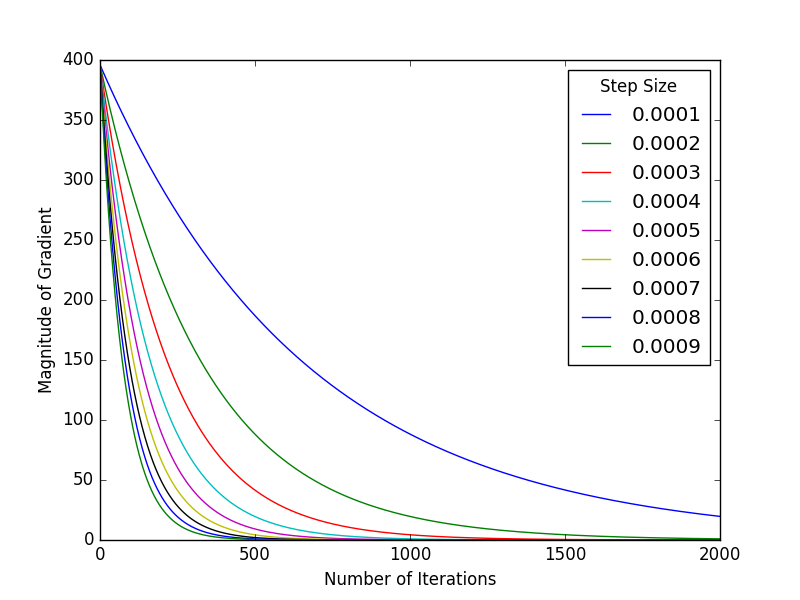
\includegraphics[width=0.5\textwidth]{../images/quadratic_steps_vs_mag}
  \caption{As the step size increases, the algorithm converges quicker.}
\end{figure}

In addition, the step size and threshold control the accuracy of the gradient descent. As step size decreases, we expect a more accurate result because the function of the initial guess over time is smoother. Similarly, as the threshold decreases, we expect a more accurate result because the algorithm needs to run for longer before reaching a stable equilibrium. To verify these claims, we run gradient descent using a two-dimensional Gaussian with mean $(10, 10)$. As we vary $\lambda$ and $\delta$, we plot the least-squares error between the returned value and the actual optimum of $(10, 10)$ (see Figure 2). Indeed, the error decreases as $\lambda$ and $\delta$ decrease.

\begin{figure}[ht!]
  \centering
    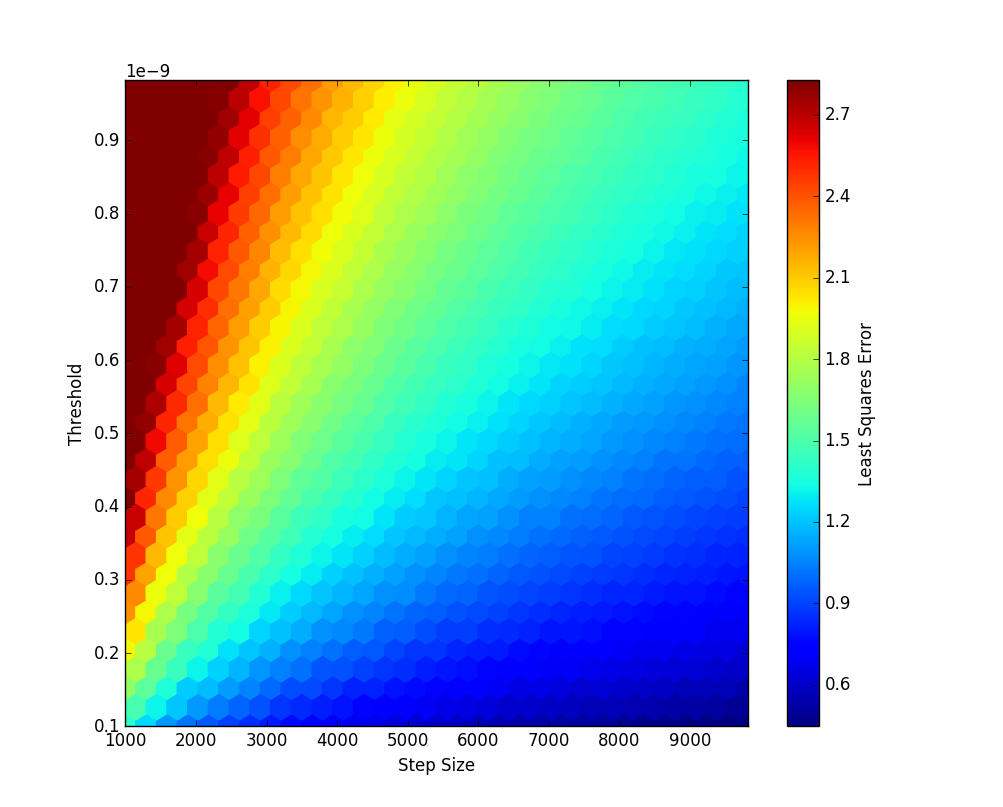
\includegraphics[width=0.5\textwidth]{../images/lsq_error_gradient}
  \caption{As $\lambda$ and $\delta$ decrease, error decreases.}
\end{figure}

Finally, we observe the affect of the initial case on the rate of convergence. When running gradient descent on a two-dimensional Gaussian with mean $(10, 10)$, one would expect that as the intial guess appraoches the optimal value, the convergence rate increases. Indeed, running the algorithm with $\lambda = 1000$ and $\delta = 10^{-11}$, we notice that the rate of convergence is much higher as the initial guess approaches the actual value (see Figure 3). 

\begin{figure}[ht!]
  \centering
    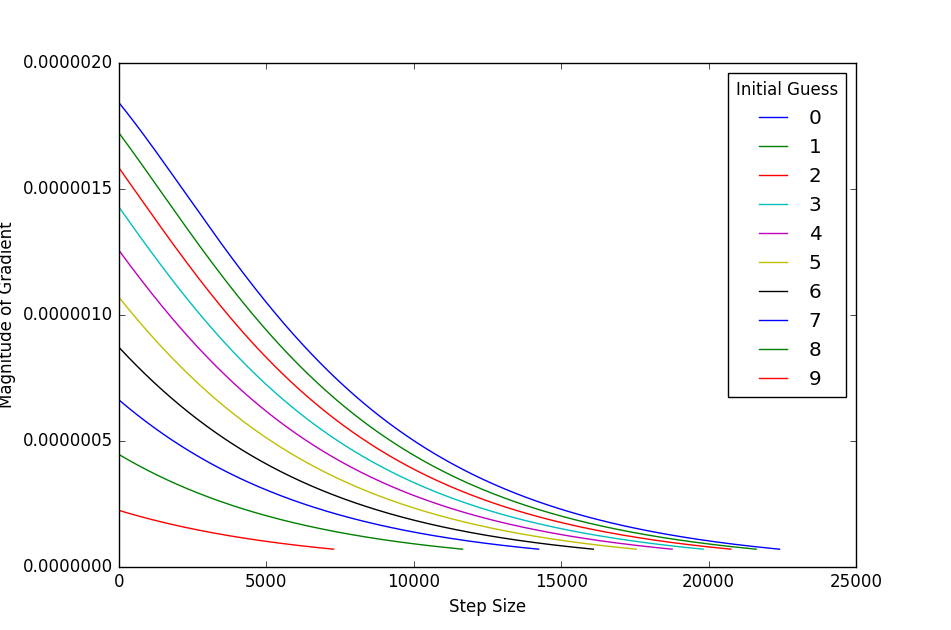
\includegraphics[width=0.5\textwidth]{../images/guess_vs_mags_2}
  \caption{As $\mathbf{x}_0$ appraoches $(10, 10)$, the rate of convergence increases.}
\end{figure}

\subsection{Stochastic Gradient Descent}



\subsection{Effect of Finite Gradient}

When the objective function doesn't have a closed form solution, one can approximate the gradient using a central finite difference. In other words, we have 
\begin{align*}
\nabla f(x) \approx \nabla_h[f](x) \dfrac{f(x+h/2) - f(x-h/2)}{h}
\end{align*}
Therefore, we only need the objective function to approximate the gradient. Note that as $h$ approaches zero, this approaches the actual value of the gradient; and has $h$ approaches infinity this value diverges. Figure 4 illustrates the impact of $h$ on the accuracy of the gradient: for small enough $h$, the approximation is accurate to several orders of magnitude.

\begin{figure}[ht!]
  \centering
    \begin{tabular}{c | c}
    $h$  & $\nabla_h[f](x)$ \\	\hline
	0.01 & $-3.1704 \cdot 10^{-7}$ \\
	0.1 & $-3.1704 \cdot 10^{-7}$ \\
	1.0 & $-3.1696 \cdot 10^{-7}$ \\
	10.0 & $-3.0923 \cdot 10^{-7}$ \\
	100.0 & $-2.6198 \cdot 10^{-8}$ \\
	1000.0 & $\approx 0$ \\
    \end{tabular}
  \caption{As $h$ increases, the accuracy of the central finite difference decreases. The actual gradient value is $-3.1704 \cdot 10^{-7}$.}
\end{figure}

\end{document}

